This section discusses the results of policy hill-climbing.

\subsubsection{1 predator vs. 1 prey}
With policy hill-climbing it is possible to pass a step size, which is a value between 0 and 1. The step size determines how radically the Q-values are updated. A low step size leads to slow changes in Q-values, whereas a high step size changes the Q-values quite radically. The effects of this step size are researched in the 1 predator versus 1 prey scenario. This is displayed in figure \ref{phc_1v1_steps}.

\begin{center}
	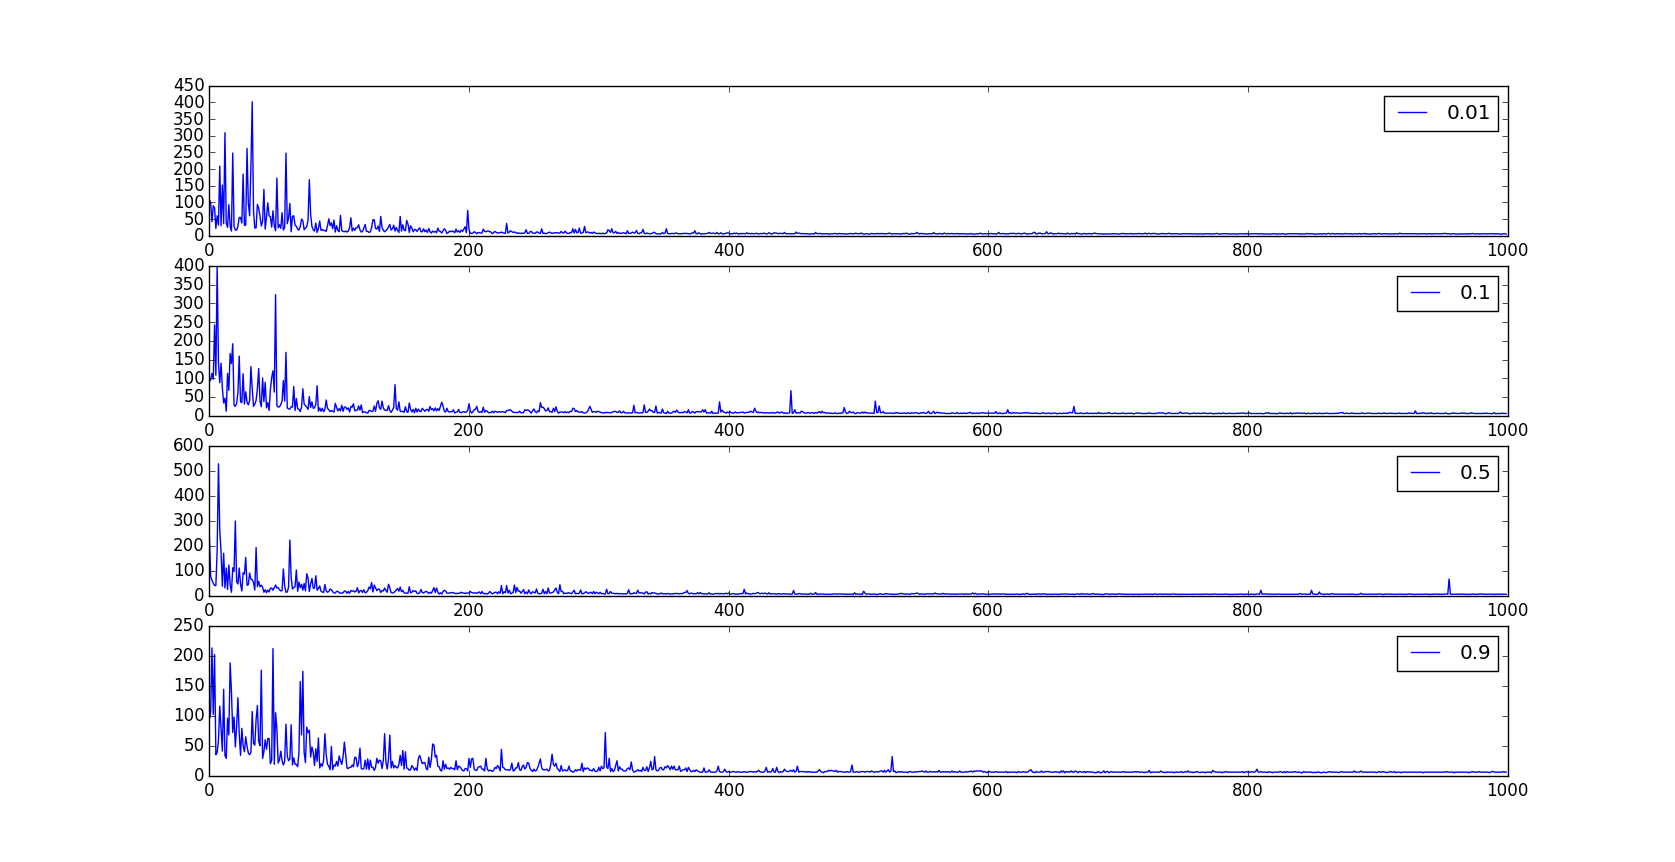
\includegraphics[scale=0.3]{allplots_hillclimbing}
	\captionof{figure}{Policy Hill-Climbing: 1 predator versus 1 prey, with varying step sizes}
	\label{graph:phc_1v1_steps}
\end{center}

The graph shows that all chosen step sizes start off quite radically. Eventually, all algorithms converge. The stepsize of 0.9 takes longest to stabilize and the most amounts of rounds to catch the prey after stabilizing. As stated before, this is a quite radical update of the Q-values. In this case, this result is not optimal. The lowest step size shows that the Q-values are hanged gradually, but still quickly. Contrary to the larger step-sizes, this is quite stable for the lowest step size. All step sizes tend to have peaks in rounds needed to catch the prey, after stabilizing. The peaks at the lowest step size are smallest. Also, number of rounds needed to catch the prey are lowest. Therefore, it seems that small step sizes are best.